\documentclass{article}

\usepackage[education,final,nonatbib]{neurips_2026}
\usepackage[utf8]{inputenc}
\usepackage[T1]{fontenc}
\usepackage{hyperref}
\usepackage{url}
\usepackage{booktabs}
\usepackage{microtype}
\usepackage{xcolor}
\usepackage{enumitem}
\usepackage{array}
\usepackage{graphicx}
% Without this, hyperref draws a coloured box around every link.
\hypersetup{colorlinks=true, linkcolor=black, citecolor=black,
            urlcolor=[rgb]{0.11,0.32,0.55}}
\setlist[itemize]{leftmargin=*,nosep,topsep=1pt}
\renewcommand{\arraystretch}{0.95}

\title{Teaching Generalizable Cooperation in Multi-Agent Reinforcement Learning}

\author{%
  Similoluwa Okunowo\\
  African Institute for Mathematical Sciences (AIMS) South Africa\\
  \texttt{similoluwa@aims.ac.za}\\
}

\newcommand{\resourceurl}{\href{https://rexsimiloluwah.github.io/marl-for-cooperative-environments/}{marl-for-cooperative-environments}}
\newcommand{\repourl}{\href{https://github.com/rexsimiloluwah/marl-for-cooperative-environments}{GitHub repository}}

\begin{document}
\maketitle

\begin{abstract}
We present an open-source, multimodal educational resource for generalizable cooperation in multi-agent reinforcement learning (MARL): how agents coordinate, communicate, and adapt when partners, communication conventions, or deployment conditions differ from training. The resource uses structured, bite-sized lessons, animated explainers, interactive practice, virtual and practical Jupyter notebooks, to move learners from cooperative MARL foundations to advanced topics like cross-play, unseen-partner evaluation, ad hoc teamwork, and zero-shot coordination. It culminates in the emerging frontier of learned collaboration among LLM agents, where the same questions of coordination and adaptation reappear.

\vspace{5pt}
{\raggedright\noindent\textbf{Tutorial website:}
\href{https://rexsimiloluwah.github.io/marl-for-cooperative-environments/}%
{rexsimiloluwah.github.io/marl-for-cooperative-environments}\par}
\end{abstract}

\vspace{-4pt}\section{Concept}

In multi-agent reinforcement learning (MARL), where multiple agents learn to
act toward a shared goal, \textbf{generalizable cooperation} asks whether
effective teamwork can persist when partners, communication conventions, or
deployment conditions differ from training. This matters in robotics, autonomous vehicles, network
optimization, and resource allocation, and increasingly in learned
collaboration among LLM agents.

This resource teaches MARL in cooperative environments through a guided learning journey rather than as a set of fragmented topics. It begins with single-agent reinforcement learning, builds through coordination and communication, then reaches partner adaptation, zero-shot teamwork, and the frontier of LLMs as cooperative agents.

\begin{center}
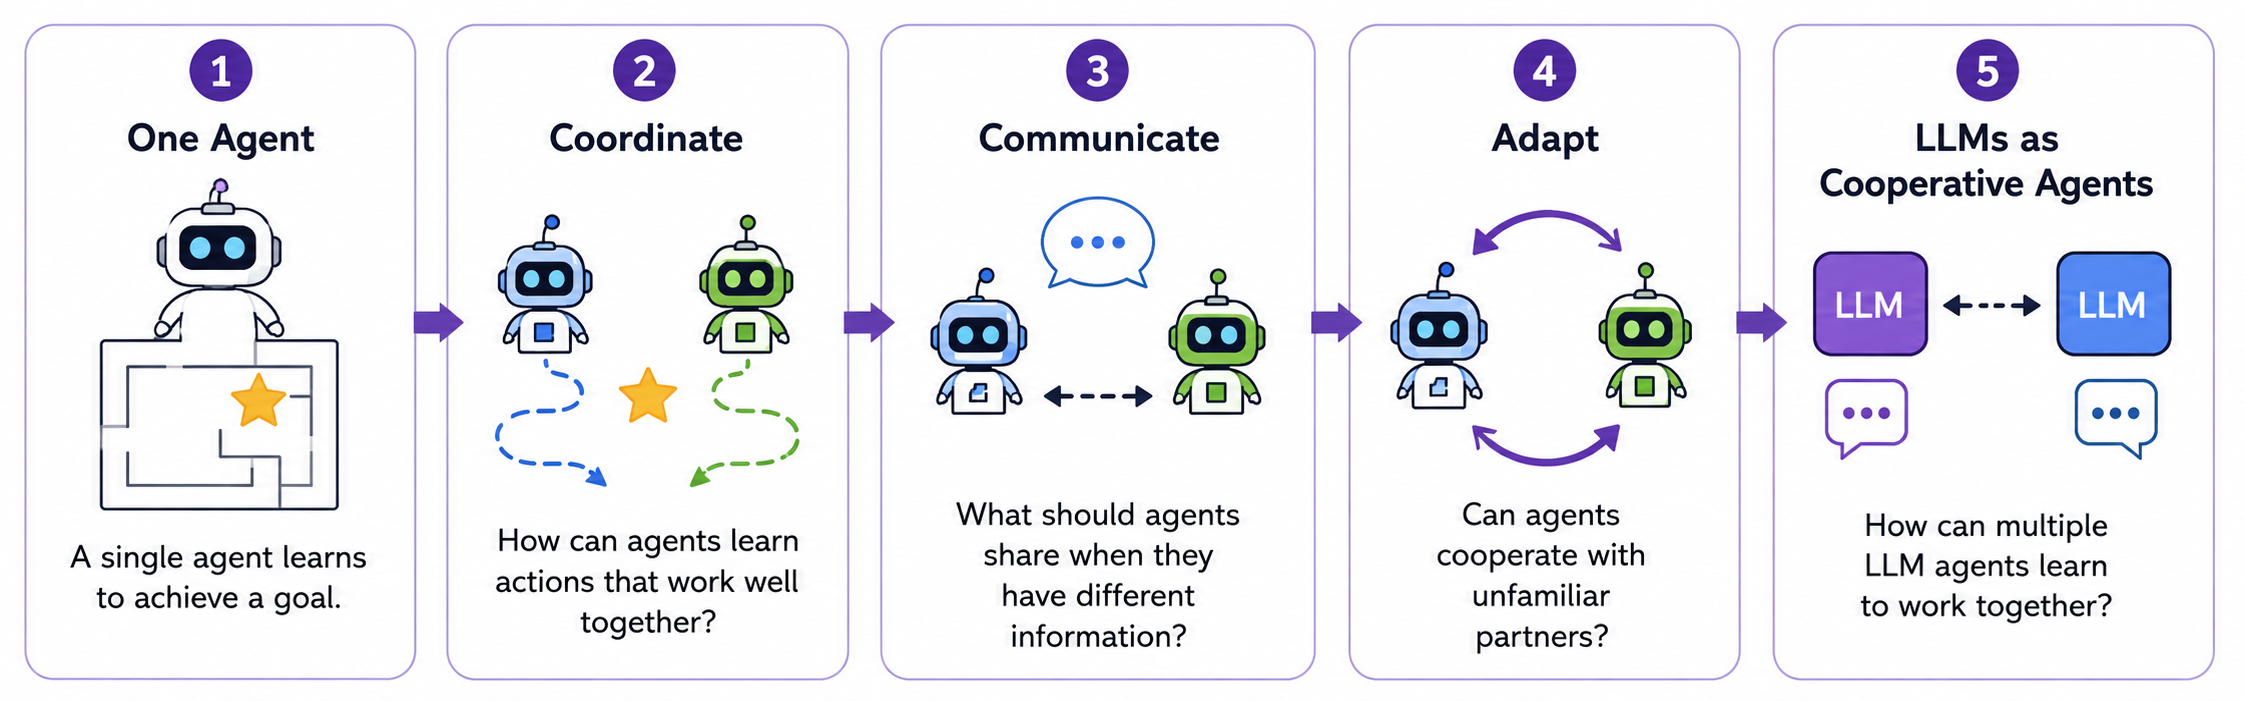
\includegraphics[width=0.97\linewidth]{figures/main.png}
\end{center}
\vspace{-8pt}
\refstepcounter{figure}\label{fig:journey}
{\footnotesize\noindent\textbf{Figure \thefigure:} The five stages of the
journey. Each challenge is created by the one before it.\par}
\vspace{4pt}

\vspace{-4pt}\section{Audience and Prerequisites}

Advanced undergraduate and graduate learners with basic reinforcement learning,
Python, probability, and linear algebra; no prior MARL required. The textbook by
Albrecht et al.~\cite{marlbook} is a useful companion for broader coverage.

\vspace{-4pt}\section{Learning Objectives}

The resource follows Bloom's Taxonomy, progressing from understanding core
concepts to applying, analysing, evaluating, and creating cooperative
multi-agent systems.
\begin{itemize}
  \item \textbf{Understand:} explain coordination, communication, credit
    assignment, CTDE, and partner dependence.
  \item \textbf{Apply:} use and compare cooperative learning approaches in
    small environments.
  \item \textbf{Analyse and Evaluate:} diagnose failures under communication
    limits and changing partners.
  \item \textbf{Create:} design and justify a cooperative MARL system that
    generalizes beyond its training partners.
\end{itemize}

\vspace{-4pt}\section{Teaching Materials}

The resource uses a multimodal learning design, combining structured
explanation, visual storytelling, retrieval practice, and hands-on
experimentation.

\begin{center}
\footnotesize
\setlength{\tabcolsep}{5pt}
\renewcommand{\arraystretch}{1.15}
\begin{tabular}{p{0.27\linewidth}p{0.655\linewidth}}
\toprule
\textbf{Teaching material} & \textbf{What it provides}\\
\midrule
Interactive tutorial website & Structured, bite-sized lessons with intuitive explanations, equations, research connections, flashcards, embedded knowledge checks, and interactive worksheets.\\
Explainer videos & Two animated explainers, on the core MARL journey (\href{https://youtu.be/TOJrFLJHXkM}{youtu.be/TOJrFLJHXkM}) and on LLMs as cooperative agents (\href{https://youtu.be/P5OAe5XLmzc}{youtu.be/P5OAe5XLmzc}).\\
Labs & In-browser virtual labs and Colab notebooks for hands-on practice with coordination, communication, partner generalization, and wireless network resource allocation.\\
\texttt{cooperative-marl-labs} & Open-source Python package with reusable environments, agents, partner policies, training utilities, evaluation tools, and visualizations.\\
\bottomrule
\end{tabular}
\end{center}

{\raggedright\noindent All teaching materials and source code are available in
the GitHub repository:
\href{https://github.com/rexsimiloluwah/marl-for-cooperative-environments}%
{github.com/rexsimiloluwah/marl-for-cooperative-environments}\par}


\vspace{-4pt}\section{Linked Recent Papers}

The learning path is grounded in recent work from 2022 to 2026 that
demonstrates the concept is active at the research frontier.

\begin{center}
\scriptsize
\setlength{\tabcolsep}{4pt}
\begin{tabular}{p{0.26\linewidth}p{0.67\linewidth}}
\toprule
\textbf{Learning question} & \textbf{Recent papers using the concept}\\
\midrule
Evaluating coordination & SMACv2~\cite{smacv2}, NeurIPS Datasets and Benchmarks 2023.\\
Learned communication & LangGround~\cite{langground}, NeurIPS 2024.\\
Unfamiliar partners & N-Agent Ad Hoc Teamwork~\cite{naht}, NeurIPS 2024; ZSC-Eval~\cite{zsceval}, NeurIPS Datasets and Benchmarks 2024.\\
LLM collaboration & MAPoRL~\cite{maporl}, ACL 2025; LLM Collaboration with MARL~\cite{llmcollab}, AAAI 2026.\\
\bottomrule
\end{tabular}
\end{center}

\vspace{-8pt}
{\scriptsize
\begin{thebibliography}{9}\setlength{\itemsep}{0pt}\setlength{\parskip}{0pt}
\bibitem{marlbook} S.~V.~Albrecht, F.~Christianos, and L.~Sch\"afer. \emph{Multi-Agent Reinforcement Learning: Foundations and Modern Approaches}. MIT Press, 2024. \href{https://www.marl-book.com}{marl-book.com}.
\bibitem{smacv2} B.~Ellis et al. SMACv2: an improved benchmark for cooperative MARL. \emph{NeurIPS Datasets and Benchmarks}, 2023.
\bibitem{langground} H.~Li et al. Language grounded MARL with human-interpretable communication. \emph{NeurIPS}, 2024.
\bibitem{naht} C.~Wang et al. N-agent ad hoc teamwork. \emph{NeurIPS}, 2024.
\bibitem{zsceval} X.~Wang et al. ZSC-Eval: a benchmark for multi-agent zero-shot coordination. \emph{NeurIPS Datasets and Benchmarks}, 2024.
\bibitem{maporl} C.~Park et al. MAPoRL: multi-agent post-co-training for collaborative LLMs with RL. \emph{ACL}, 2025.
\bibitem{llmcollab} S.~Liu et al. LLM collaboration with multi-agent reinforcement learning. \emph{AAAI}, 2026.
\end{thebibliography}}

\vspace{2pt}
\begin{center}
\fcolorbox{black!25}{black!4}{%
\begin{minipage}{0.955\linewidth}
\scriptsize
\textbf{AI Usage and Educational Integrity.} Generative AI tools supported
parts of the writing, coding, visual design, and iteration of the resource. All
educational content and technical claims were reviewed before inclusion.
Simplified environments in the Python package are designed for teaching and
experimentation, \textbf{not for evaluating or comparing MARL algorithms for
scientific claims}. The resource is \textbf{actively maintained and will
continue to be updated as the field evolves and learner or instructor feedback
is incorporated}.
\end{minipage}}
\end{center}

\end{document}
